\documentclass[11pt]{lecture}

% \usepackage{chronology} %% for timeline
\def\fullsize{0.55\textwidth}

\usepackage{xcolor}
\hypersetup{
    colorlinks,
    linkcolor={red!50!black},
    citecolor={blue!50!black},
    urlcolor={blue!80!black}
}

\usepackage{booktabs}
\usepackage{multirow}

\begin{document}

\course{CS 6210/CS 4210 ADVANCED OPERATING SYSTEMS}
\title{Distributed File System (Part 0)}%\footnotemark[1]\footnotemark[2]
\semester{Fall 2017}
\instructor{Prof. Umakishore Ramachandran}
\author{Long Gong}
\footnotetext[1]{All the figures in this scribe are directly from or modified from the lecture slides provided by 
Prof. Umakishore Ramachandran.}
\maketitle

\section{Overview}\label{sec: overview}

In this lecture, we will cover several background technologies for distributed file system.



\section{Motivation}\label{sec: mot}

Before starting talking about distributed file system, 
let us first review the network file system. 

\noindent
{\bf Network File System (NFS).} Network file systems (NFS)~\cite{nfs} has evolved over time, 
but the idea is still the same. As shown in~\autoref{fig: nfs}, in NFS, you have clients that 
are distributed all over the local area network, and you have file servers sitting on the 
local area network. These file servers are central so far as each client is concerned. 
The system administrator may partition these servers, say there is one server that 
is designated for a certain class of users. For instance, if you take a university setting, it 
might have one server serving all the faculty's needs, and maybe another server 
serving all the students' needs. But so far as a single client is concerned, it is still a 
centralized view, access to a central server over local area network. Since the 
disk being electromagnetic is slow, the serve will cache the files that it retrieves from 
the disk in memory, so that it can serve the clients better by serving it out of the file cache that 
is in memory rather than going to the disk. \autoref{fig: nfs} is a typical structure of 
a network file system. A centralized server which is used in NFS is a serious 
bottleneck for scalability. A single server has to field the client requests coming from 
the group of users that it is serving and manage all the data and metadata for all the files 
that are host on this particular server. The data and metadata of files are persistent 
data structures~\cite{persistentds} and therefore the file server has to access these data structures over the I/O 
bus which is available for talking to the disk subsystem. So with a centralized view like this, 
there is limited bandwidth that is available for the server to get the data and metadata 
in and out of the disk. The file system cache is also limited because it is confined to 
the memory space that is available in a given server. So instead of this centralized view of 
the file system, {\it can we implement the file system in a distributed manner ?}

\begin{figure}[!htb]
\centering
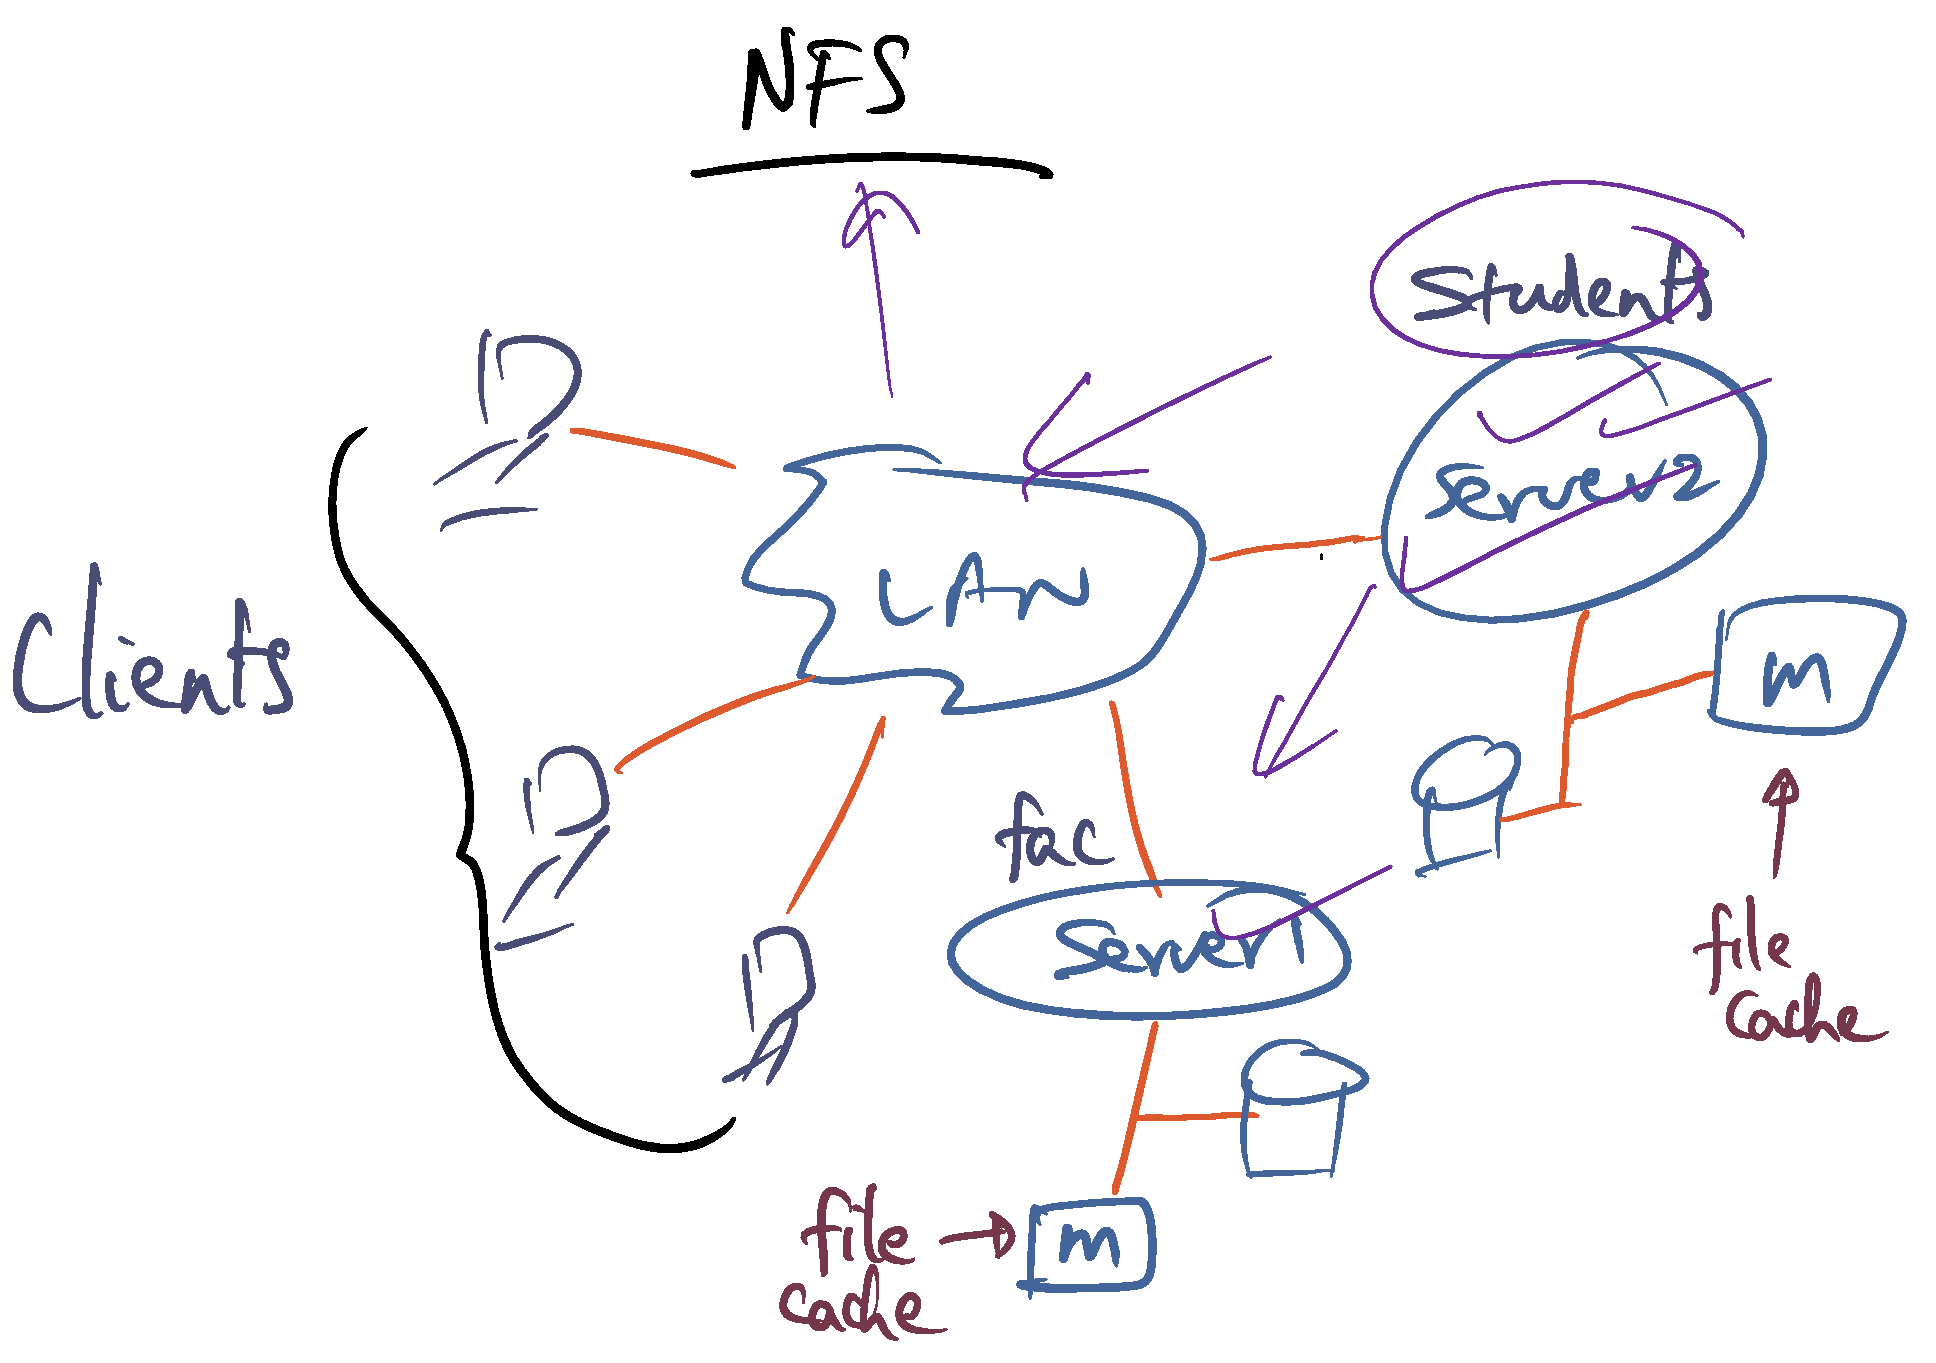
\includegraphics[width=\fullsize]{Figures/nfs}
\caption{A typical structure of network file system.}\label{fig: nfs}
\end{figure}

\noindent
{\bf Distributed File System (DFS).} The vision with a distributed file server is that there 
is no central server anymore. Each file is distributed across several servers. We want to take a 
file and distribute it across several different nodes in local area network. Since the DFS 
is implemented across all the disks in the network, if a client wants to read or write a 
file, then it actually is contacting all the servers potentially to get the data that is 
looking for. As each file is distributed across all the servers in the DFS, the I/O bandwidth 
that is available cumulatively across all of these servers can be used to serve the needs of every 
individual client. Also, this allows distributing the management of the metadata that is 
associated with the files among the server nodes that are available. Furthermore, we have 
more memories available in all these servers. Which means we have a bigger memory footprint available 
for implementing a file cache including all of the server memories plus the memory that 
may be there in the clients as well. That is where we can actually go towards cooperative caching 
among the clients as well. So in the extreme we treat all the nodes in the cluster equally. That is 
all of them have interchangeable roles as clients or servers. Therefore, we can make this 
DFS a serverless file system~\cite{AndersonXFS} if we allow the responsibility of managing the files, serving the 
files, caching the files equally distributed among all the nodes of the cluster.


\section{Background Technologies}\label{sec: background}

Before starting details on distributed 
file system. We have to first review certain background technologies.

\begin{figure}
\centering
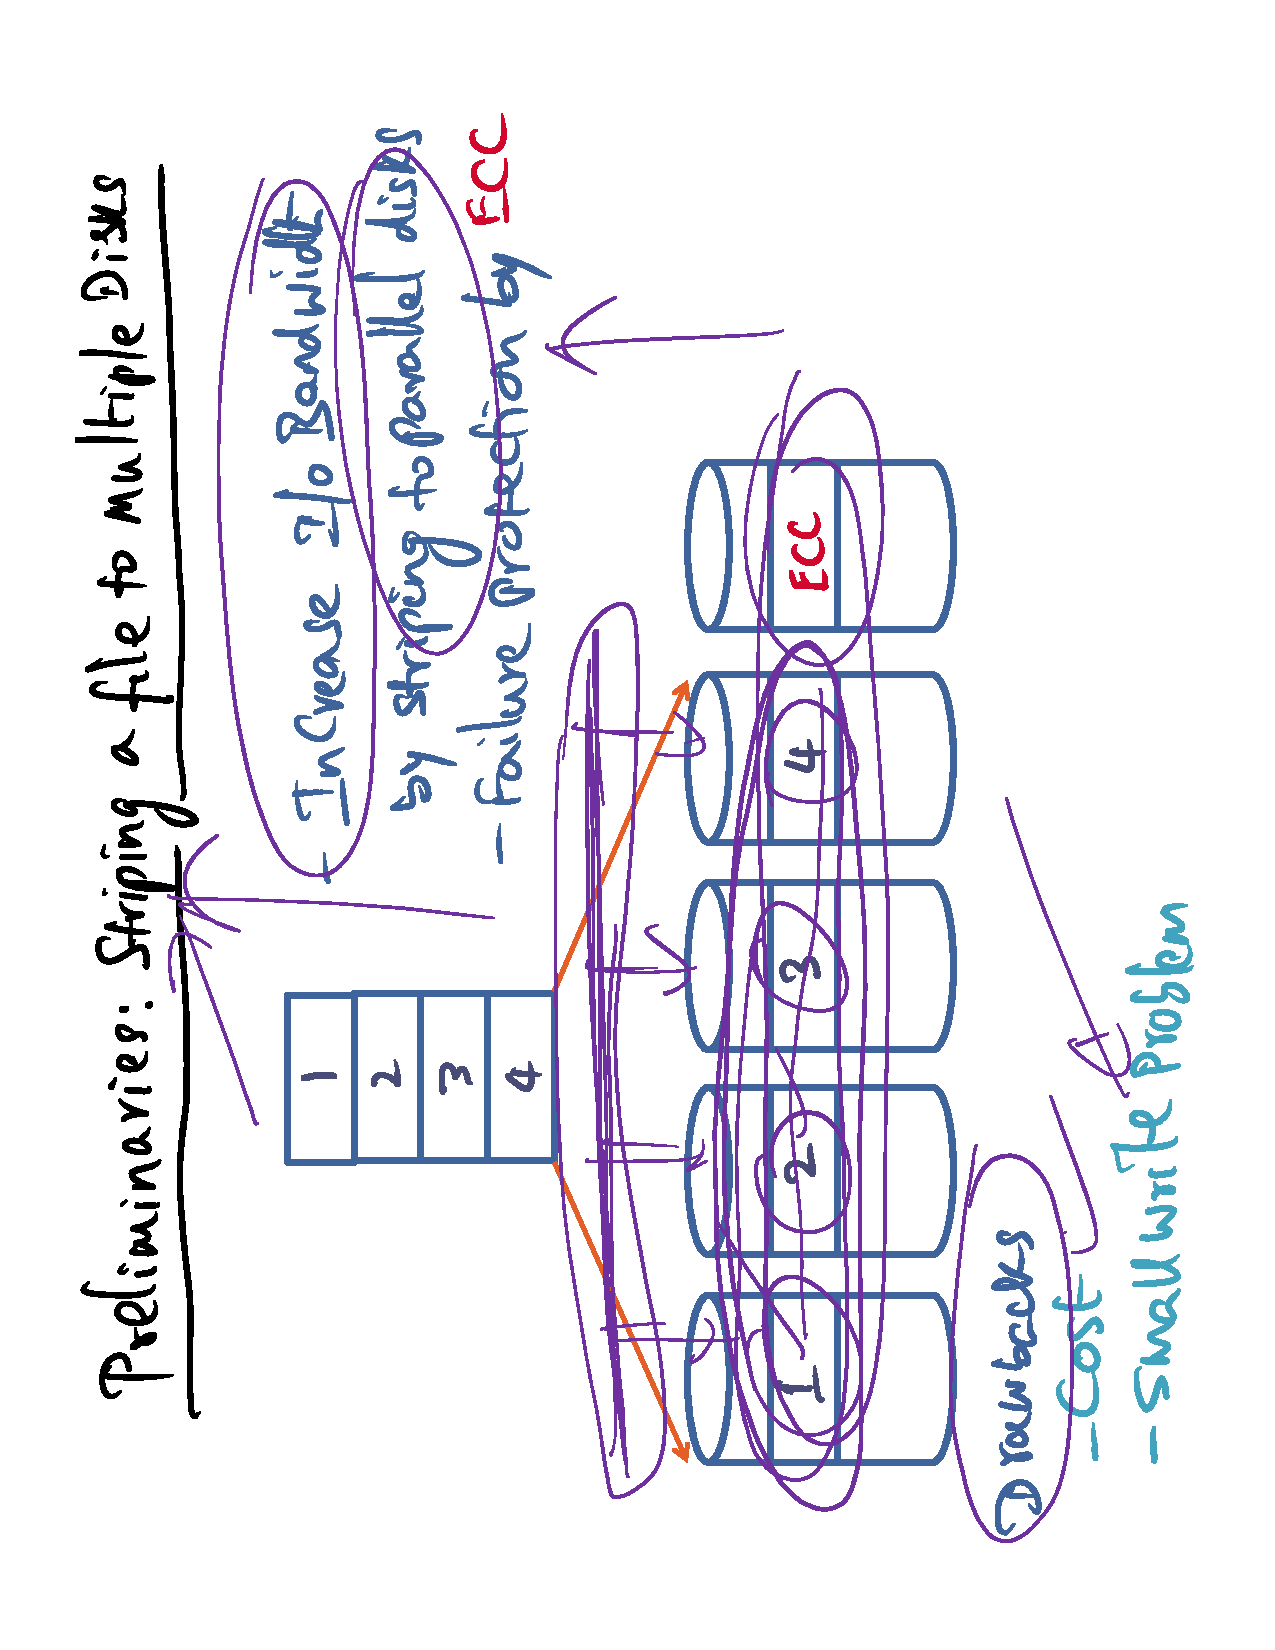
\includegraphics[width=\fullsize, angle=-90]{Figures/striping-file}
\caption{Stripping a file to multiple disks.}\label{fig: stripping}
\end{figure}
\noindent
{\bf Stripping a File to Multiple Disks.} The first background technology is RAID storage. 
RAID stands for redundant array of inexpensive disks\footnote{Note that, here we use the 
original ``version'' of RAID invented in~\cite{Patterson1998RAID}. However, it is more 
common to interpret the acronym as standing for ``redundant array of independent disks". }. 
The idea is that a given disk might have certain bandwidth available, if I can string together a number of 
disks in parallel, then cumulatively I can get much more I/O bandwidth. However, as we increase 
the number of disks, we also increase the probability of failures. Therefore, in the RAID 
technology, they also use an error correcting technology. The basic idea is that, when we write a file, 
for instance, as shown in~\autoref{fig: stripping}, the file has four parts. The RAID technology will write 
part $1$ to disk $1$, part $2$ to disk $2$, and so on so forth. It also compute a checksum for this 
particular data that I have stored on the four disks, and store the checksum on a fifth disk. 
That is what is called error correcting code (ECC)~\cite{lin2004ecc}. ECC allows errors to be detected when 
we read things from the disk, and we can detect errors in it and using the ECC data on the fifth 
disk to correct the errors. That is the big picture of how stripping of file to multiple disks works. 

The drawback of this RAID technology is first of all the cost, since we have to have multiple hardware 
drives in order to store a single file. The second problem is small write problem. That is if my file is 
really really small, then parts of this file will be written to multiple disks. That is inefficient in terms of 
how you store data. The reason why it is inefficient is that in order to read this small file which 
has been stripped to multiple disks, we have to get data from all these disks. That is why it is detrimental about 
the hardware RAID in terms of handling a normal file system that may have a population of small files and 
large files and so on an so forth. But the idea of having an array of disks to serve the file 
system is indeed a good one because it increases the overall bandwidth that is available in the server. 

\noindent
{\bf Log Structured File System.} That brings us another technology, which is called log structured 
file system. The idea is as follows. When I made a change to a file meaning that I either append to 
the file or make some modifications. Rather than writing the file as is, I am going to write the 
change that I made to the file as a log record. So, I have a log record that says, what are the changes I made 
to say the file {\code x}. Similarly, I have log record for the changes I made to file {\code y}. This is 
being done in a data structure which is called log segment. And we keep this log segment data structure 
in memory to make it fast in terms of the file system operation. With the log segment data structure, 
what we can do is to buffer the changes to multiple files in one contiguous log segment data structure. 
Because the log segment is contiguous, we can write it sequentially on the disk. And sequential writes 
to disk are good in the disk subsystem. Every once a while we will flush the log segment to disk, 
once this log segment fills up to a certain extent, or periodically. And the reason is the fact that 
we have to worry about the reliability of the file system once some node crashes. Clearly, this solves the 
small write problem. Note that in this log structured file system, there are only logs, no data files. 
You will never write any data files. When you have to read a file, it has to go to the disk and 
fetch the file and the file system has to reconstruct the file from the logs that it has stored on 
the disk. Once it comes into the memory of the server, then in the file cache the file is going to remain as 
a file. But if at any point, the server has to fetch the file from the disk, it is actually fetching the 
log segments and then reconstructing the file. That is important. Because it indicates that in a 
log structured file system, there could be latency associated with reading a file for the first 
time from the disk. Since you have to read all the log segments and reconstruct the file. That is 
where parallel RAID technology can be very helpful, because you are aggregating all the bandwidth that 
is available for reading the log segments from multiple disks at the same time. 

Note that, the logs are going to have lots of holes creating by overwriting the same block of 
a particular file. So in a log structured file system, the logs have to be cleaned periodically 
to ensure that the disk cluttered with wasted logs that have empty holes in them because of old 
writes to parts of a file that are not longer relevant. 


\noindent
{\bf Software RAID.} The next background technology is software RAID. As mentioned above, hardware 
RAID has two problems: The first problem is small write and the second problem is employing 
multiple hardware drives. Generally speaking, hardware RAID is very expensive. In a local 
area network, we have a lot of computational power distributed over the LAN and every node on the LAN 
has associated with it are disks. So {\it could we not use the disks for doing exactly the same thing that 
we did with hardware RAID ?} That is to stripe a file across the disks of all the nodes that are in the LAN. 
That is the idea behind the zebra file system~\cite{Hartman1994Zebra} that was built at UC Berkeley which was the first one 
to experiment with this software RAID technology. It combines both the log structured file system 
and the RAID technology. That is it actually stripes the log segments into different nodes in the LAN. 
Therefore, it solves the small write problem and obtains the advantages of parallelism from RAID. 

\noindent
{\bf xFS.} Now, it is the time to put all together and plus some more, resulting in a particular 
distributed file system, which is called xFS~\cite{AndersonXFS}. xFS is also built by UC Berkeley. xFS builds upon 
several prior technologies. The first one is the log based stripping that was used in zebra file system. 
Another technology called cooperative caching which is also a prior UC Berkeley project. And in addition, 
xFS also introduced several new nuances to make the distributed file system truly scalable. These 
techniques include dynamic management of data and metadata, subsetting of the storage servers, and 
distributed log cleaning. And all the techniques would be covered in more details in the next lecture. 





\bibliographystyle{IEEEtran}
\bibliography{references}


\end{document}
